% Provenance (never printed): see sources/outline_sources.md (Year 1: the general
% circulation of the atmosphere, Hadley, Ferrel and polar cells, the ITCZ, Walker cells,
% jet streams, the geostrophic wind, depressions and anticyclones). Exercise and problem
% values in the Book 3 scratch calculator calc/ch28.py; figures from
% figdata/bachelor-1/angular_momentum_wind.py, weather_map.py (an invented map) and
% general_circulation.py (NCEP-NCAR Reanalysis 1, long-term means 1991-2020, datasets
% bachelor-1-ncep-{uwnd-p,vwnd-p,uwnd-sfc,slp,prate-monthly}).
% Physics owns the Coriolis force and the hydrostatic relation (recalled). Book 1 (g8) gave
% the global winds, the convection cell, depressions and anticyclones, isobars and the
% rotation of the wind around them, in words: re-founded here with forces and data.
% ENSO and the monsoons are the Year 2 volume's; the thermal wind the Year 3 volume's.
\chapter{A circulação geral da atmosfera}\label{ch:b1:atmospheric-circulation}

Os veleiros que cruzavam da Europa e da África para as Américas dependiam dos ventos \omterm{def:b1:atmospheric-circulation:winds}{alísios},
leste constantes dos trópicos. Mais perto do equador, a cerca de cinco graus dele, os mesmos ventos
se extinguiam, no cinturão de calmarias e aguaceiros persistentes que os marinheiros chamavam de
doldrums. Muito acima de ambos, a cerca de nove quilômetros de altura, estreitos rios de ar
chamados \omterm{def:b1:atmospheric-circulation:jet}{correntes de jato} podem soprar a mais de \qty{440}{km/h}. Este capítulo explica os três:
por que o ar que se move sobre um planeta em rotação acaba soprando ao longo das isóbaras em vez de
através delas, como o excedente dos trópicos aciona uma grande célula de circulação em cada lado do
equador, e por que o ar que deixa o equador em altitude se transforma em um jato de oeste.
% ledger: nos:trade-winds, nos:doldrums, noaajs:jet

\begin{omfigure}
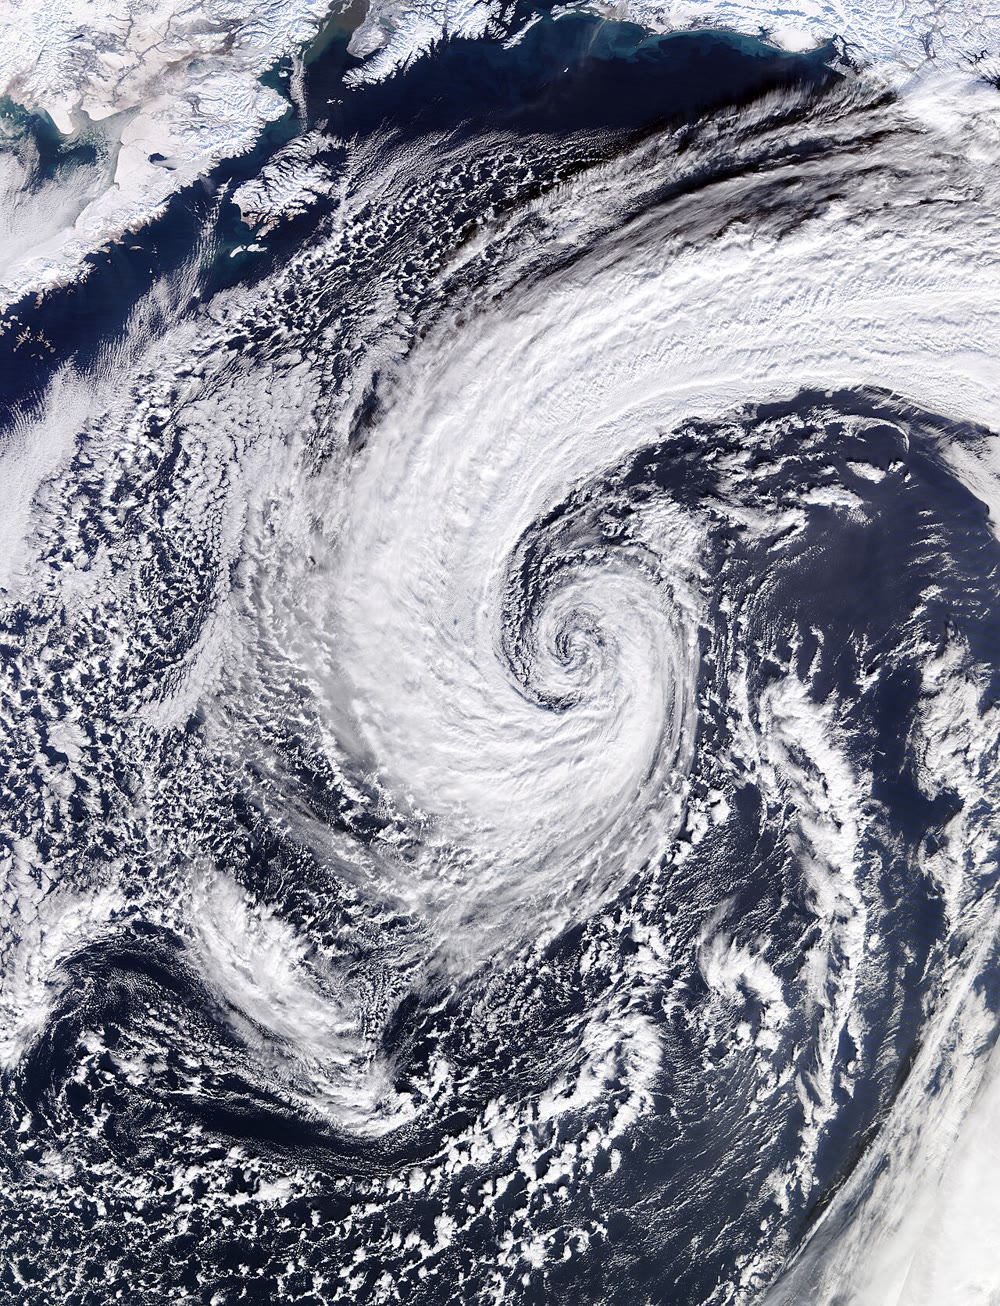
\includegraphics[width=0.5\linewidth]{images/book3/b1-alaska-low.jpg}

{\small Um \omterm{def:b1:atmospheric-circulation:cyclone}{ciclone} extratropical sobre o Golfo do Alasca em 28 de janeiro de 2018, visto pelo
instrumento MODIS a partir da órbita; a costa do Alasca, coberta de neve, está no alto à esquerda, e
o norte está aproximadamente para cima. As faixas de nuvem se enrolam em sentido anti-horário em
direção ao centro, como faz o ar de uma depressão do Hemisfério Norte. (NASA, MODIS/LANCE, domínio
público, via Wikimedia Commons.)}
\label{fig:b1:atmospheric-circulation:alaska}
\end{omfigure}
% ledger: commons:alaska-low, nws:cyclone

\begin{recall}
Os livros de física dão a relação hidrostática e a força de Coriolis: em um referencial que gira com
velocidade angular $\vec\Omega$, um corpo de massa $m$ que se move com velocidade $\vec v$ em
relação ao referencial sente a força fictícia $-2m\,\vec\Omega\times\vec v$, em ângulo reto com seu
movimento. Para a Terra, $\Omega = 2\pi/T_\star$ com o dia sideral $T_\star = \qty{23.9345}{h}$, isto
é $\Omega = \qty{7.292e-5}{rad.s^{-1}}$. O Livro~1 descreveu os ventos globais (os \omterm{def:b1:atmospheric-circulation:winds}{alísios}, os
\omterm{def:b1:atmospheric-circulation:winds}{ventos de oeste}, os leste polares), a célula de convecção, as depressões e \omterm{def:b1:atmospheric-circulation:cyclone}{anticiclones}, as isóbaras
de um mapa do tempo e o giro do vento em torno dos centros. \Cref{ch:b1:fluid-envelopes-structure}
deu a \omterm{def:b1:fluid-envelopes-structure:standard-atmosphere}{atmosfera padrão} e o \omterm{def:b1:fluid-envelopes-structure:lapse-rate}{gradiente adiabático seco}, e \cref{ch:b1:radiation-heat-transport} o
transporte de calor para os polos que a circulação leva.
% ledger: earth:Trot, nws:coriolis
\end{recall}

\section{Forças sobre o ar em movimento}\label{sec:b1:atmospheric-circulation:forces}

Uma \omterm{def:b1:fluid-envelopes-structure:parcel}{porção de ar} é empurrada pela pressão do ar em volta, puxada pela gravidade, freada pelo atrito
perto do solo e, vista da Terra em rotação, desviada pela força de Coriolis. A gravidade e a força
de pressão vertical se equilibram quase exatamente: é a relação hidrostática. O tempo é feito pelas
forças que restam na horizontal.

\begin{definition}[Força do gradiente de pressão]\label{def:b1:atmospheric-circulation:pgf}
A \emph{força do gradiente de pressão}\index{força do gradiente de pressão} é a força resultante
exercida sobre uma porção de fluido pela pressão do fluido em volta. Por unidade de massa ela é
$-(1/\rho)\nabla p$, em que $\rho$ é a densidade e $\nabla p$ o gradiente de pressão: aponta de alta
para baixa pressão, através das isóbaras.
\end{definition}
% ledger: nws:geostrophic

\begin{proposition}[A força do gradiente de pressão]\label{prop:b1:atmospheric-circulation:pgf}
Sobre uma porção de volume $\mathrm dV$ e densidade $\rho$, a pressão do fluido circundante exerce a
força $-\nabla p\,\mathrm dV$, uma aceleração $-(1/\rho)\nabla p$.
\end{proposition}

\begin{proof}
Tome uma pequena caixa de arestas $\mathrm dx$, $\mathrm dy$, $\mathrm dz$ ao longo dos eixos. Em
sua face em $x$, a pressão empurra na direção $+x$ com a força
$p(x)\,\mathrm dy\,\mathrm dz$; em sua face em $x + \mathrm dx$, na direção $-x$ com $p(x + \mathrm dx)\,\mathrm dy\,\mathrm dz$. A força líquida ao longo de $x$ é $[p(x) - p(x + \mathrm dx)]\,\mathrm dy\,\mathrm dz = -(\partial p/\partial
x)\,\mathrm dV$, e analogamente ao longo de $y$ e $z$. O total é $-\nabla p\,
\mathrm dV$; dividindo pela massa $\rho\,\mathrm dV$ obtém-se a aceleração.
\end{proof}

Uma pressão uniforme não exerce força líquida: só suas diferenças empurram. Em um mapa do tempo o
gradiente horizontal é lido nas isóbaras: seu tamanho é o degrau de pressão entre duas isóbaras
dividido pela distância entre elas. Para isóbaras de \qty{4}{hPa} de distância e \qty{400}{km} de
distância ao nível do mar, onde $\rho \approx \qty{1.225}{kg.m^{-3}}$, a aceleração é $400/(1.225 \times \num{4e5}) = \qty{8.2e-4}{m.s^{-2}}$, menos de um décimo de milésimo de $g$, mas suficiente
para levar o ar do repouso a \qty{10}{m/s} em três horas e meia.
% ledger: ussa76:sea-level

O ar sente a força de Coriolis porque é observado da Terra em rotação. Sua parte horizontal depende
da \omterm{def:b1:spherical-astronomy:geographic}{latitude} por meio de um único número.

\begin{definition}[Parâmetro de Coriolis]\label{def:b1:atmospheric-circulation:coriolis-parameter}
O \emph{parâmetro de Coriolis}\index{parâmetro de Coriolis} na \omterm{def:b1:spherical-astronomy:geographic}{latitude} $\varphi$ é $f = 2\Omega\sin\varphi$,
em que $\Omega$ é a velocidade angular da Terra. É positivo no Hemisfério Norte, negativo no Sul,
zero no equador e maior nos polos, $2\Omega = \qty{1.458e-4}{s^{-1}}$.
\end{definition}
% ledger: earth:Trot

\begin{proposition}[Aceleração horizontal de Coriolis]\label{prop:b1:atmospheric-circulation:coriolis}
Para um vento horizontal $\vec v$ na \omterm{def:b1:spherical-astronomy:geographic}{latitude} $\varphi$, a parte horizontal da aceleração de Coriolis
é $-f\,\vec k\times\vec v$, em que $\vec k$ é a vertical ascendente: ela tem tamanho $|f|\,|\vec v|$ e
aponta em ângulo reto com o vento, para sua direita no Hemisfério Norte e para sua esquerda no Sul.
\end{proposition}

\begin{proof}
Use eixos locais $x$ para leste, $y$ para norte, $z$ para cima. O vetor de rotação da Terra está no
plano do meridiano, no ângulo $\varphi$ acima do horizonte norte: $\vec\Omega =
\Omega(0, \cos\varphi, \sin\varphi)$. Para $\vec v = (u, v, 0)$,
\[
  \vec\Omega\times\vec v = \Omega\,(-v\sin\varphi,\ u\sin\varphi,\ -u\cos\varphi),
  \qquad -2\vec\Omega\times\vec v = (f v,\ -f u,\ 2\Omega u\cos\varphi).
\]
Como $\vec k\times\vec v = (-v, u, 0)$, a parte horizontal $(fv, -fu)$ é $-f\,\vec k\times\vec v$. O
vetor $\vec k\times\vec v$ é $\vec v$ girado de \ang{90} no sentido anti-horário visto de cima; seu
oposto é $\vec v$ girado no sentido horário, para a direita, quando $f > 0$, e para a esquerda quando
$f < 0$.
\end{proof}
% ledger: earth:Trot

A parte vertical, $2\Omega u\cos\varphi$, vale no máximo \qty{1.5e-3}{m.s^{-2}} para um vento de
\qty{10}{m/s}, cerca de \num{1.5e-4} de $g$: o equilíbrio hidrostático a absorve. A parte horizontal,
por menor que seja, não tem rival na atmosfera livre acima da camada de atrito, e em horas ela molda
todos os ventos.

Perto do solo, o ar também roça contra a superfície. Na camada mais baixa, de um quilômetro, a
camada de atrito dos meteorologistas, o atrito muda tanto a velocidade quanto a direção do vento;
os redemoinhos turbulentos levam o arrasto da superfície para cima, e a força age aproximadamente
contra o vento e cresce com ele. Acima, na atmosfera livre, o atrito é pequeno.
% ledger: nws:friction-layer

\section{O vento geostrófico}\label{sec:b1:atmospheric-circulation:geostrophic}

\begin{definition}[Equilíbrio geostrófico, vento geostrófico]\label{def:b1:atmospheric-circulation:geostrophic}
Um escoamento horizontal está em \emph{equilíbrio geostrófico}\index{equilíbrio geostrófico} quando
sua \omterm{def:b1:atmospheric-circulation:pgf}{força do gradiente de pressão} e sua força de Coriolis se anulam. O \emph{vento geostrófico}\index{vento geostrófico}
$\vec v_g$ é o vento que realiza esse equilíbrio para um dado campo de pressão: $-(1/\rho)\nabla p - f\,\vec k\times\vec v_g = \vec 0$.
\end{definition}
% ledger: nws:geostrophic

\begin{theorem}[O vento geostrófico]\label{thm:b1:atmospheric-circulation:geostrophic}
Longe do equador,
\[
  \vec v_g = \frac{1}{\rho f}\,\vec k\times\nabla p, \qquad
  |\vec v_g| = \frac{|\nabla p|}{\rho\,|f|} .
\]
O \omterm{def:b1:atmospheric-circulation:geostrophic}{vento geostrófico} sopra ao longo das isóbaras, mais depressa onde elas estão mais próximas. No
Hemisfério Norte ele deixa a baixa pressão à sua esquerda; no Hemisfério Sul, à sua direita.
\end{theorem}

\begin{proof}
Para um vetor horizontal $\vec w$, $\vec k\times(\vec k\times\vec w) = -\vec w$. Aplicando $\vec k\times$
ao equilíbrio $f\,\vec k\times\vec v_g = -(1/\rho)\nabla p$ obtém-se $-f\vec v_g = -(1/\rho)\,\vec k\times\nabla p$,
daí a fórmula, válida onde $f \neq 0$. Como $\vec k\times\nabla p$ é perpendicular a $\nabla p$, o
vento é perpendicular ao gradiente, isto é, segue as isóbaras; seu tamanho é $|\nabla
p|/(\rho|f|)$. O vetor $\vec k\times\nabla p$ é o gradiente girado de \ang{90} no sentido
anti-horário. Olhando ao longo dele, o gradiente, que aponta para a alta pressão, fica à direita,
logo a baixa pressão fica à esquerda; para $f > 0$ o vento tem a direção de $\vec k\times\nabla p$,
para $f < 0$, a oposta.
\end{proof}

\begin{example}[Um vento lido das isóbaras]\label{ex:b1:atmospheric-circulation:geostrophic}
A \ang{50} N, $f = 2 \times \num{7.292e-5} \times \sin\ang{50} = \qty{1.117e-4}{s^{-1}}$.
Isóbaras de \qty{4}{hPa} de distância e \qty{400}{km} de distância dão $|\nabla p| = 400/\num{4e5} =
\qty{1.0e-3}{Pa.m^{-1}}$ e, com $\rho = \qty{1.225}{kg.m^{-3}}$, um \omterm{def:b1:atmospheric-circulation:geostrophic}{vento geostrófico} de
$\num{1.0e-3}/(1.225 \times \num{1.117e-4}) = \qty{7.3}{m/s}$. O mesmo espaçamento a \ang{20} N, onde
$f$ é menos da metade, daria \qty{16.4}{m/s}.
\end{example}
% ledger: earth:Trot, ussa76:sea-level

O equilíbrio não é instantâneo. O ar posto em movimento por um gradiente de pressão gira sob a força
de Coriolis à taxa $f$, cerca de uma vez a cada $2\pi/f$, cerca de dezesseis horas a \ang{50}; padrões
que duram mais que algumas horas, e são maiores que algumas centenas de quilômetros, são próximos do
geostrófico. Perto do equador $f$ tende a zero, a fórmula deixa de valer, e os ventos dos trópicos
profundos não são geostróficos.

\begin{omfigure}
\begin{tikzpicture}[>={Stealth[length=2.2mm]}, font=\scriptsize]
  % left panel: geostrophic balance
  \begin{scope}
    \draw[isobar] (-2.4,1.2) -- (2.4,1.2) node[right] {\qty{996}{hPa}};
    \draw[isobar] (-2.4,0) -- (2.4,0) node[right] {\qty{1000}{hPa}};
    \draw[isobar] (-2.4,-1.2) -- (2.4,-1.2) node[right] {\qty{1004}{hPa}};
    \node[pressure low] at (0,2.0) {L};
    \node[pressure high] at (0,-2.0) {H};
    \fill (0,0) circle (1.6pt);
    \draw[->, very thick, omThm] (0,0) -- (0,1.0);
    \node[omThm, anchor=east] at (-0.08,0.6) {gradiente de pressão};
    \draw[->, very thick, omDef] (0,0) -- (0,-1.0);
    \node[omDef, anchor=east] at (-0.08,-0.6) {Coriolis};
    \draw[->, line width=1.6pt, black] (0,0) -- (1.9,0) node[above, pos=0.75] {vento $\vec v_g$};
    \node[anchor=north] at (0,-2.4) {sem atrito: geostrófico};
  \end{scope}
  % right panel: with friction (alpha = 25 deg, V = Vg cos alpha)
  \begin{scope}[xshift=7.4cm]
    \draw[isobar] (-2.4,1.2) -- (2.4,1.2) node[right] {\qty{996}{hPa}};
    \draw[isobar] (-2.4,0) -- (2.4,0) node[right] {\qty{1000}{hPa}};
    \draw[isobar] (-2.4,-1.2) -- (2.4,-1.2) node[right] {\qty{1004}{hPa}};
    \node[pressure low] at (0,2.0) {L};
    \node[pressure high] at (0,-2.0) {H};
    \fill (0,0) circle (1.6pt);
    \draw[->, very thick, omThm] (0,0) -- (0,1.0);
    \node[omThm, anchor=east] at (-0.08,0.6) {gradiente de pressão};
    \draw[->, very thick, omDef] (0,0) -- ({1.0*cos(25)*sin(25)},{-1.0*cos(25)*cos(25)});
    \node[omDef, anchor=west] at (0.42,-0.62) {Coriolis};
    \draw[->, very thick, omMeth] (0,0) -- ({-1.0*sin(25)*cos(25)},{-1.0*sin(25)*sin(25)})
      node[below left, inner sep=1pt] {atrito};
    \draw[->, line width=1.6pt, black] (0,0) -- ({1.9*cos(25)*cos(25)},{1.9*cos(25)*sin(25)})
      node[above, inner sep=2pt] {vento $\vec v$};
    \draw[black!50, dashed] (0,0) -- (1.9,0);
    \draw[black!60] (1.0,0) arc[start angle=0, end angle=25, radius=1.0];
    \node[black!70] at (1.22,0.22) {$\alpha$};
    \node[anchor=north] at (0,-2.4) {com atrito: mais lento, cruzando as isóbaras};
  \end{scope}
\end{tikzpicture}

{\small Forças sobre uma \omterm{def:b1:fluid-envelopes-structure:parcel}{porção de ar} no Hemisfério Norte, com baixa pressão ao norte. À esquerda:
na atmosfera livre a \omterm{def:b1:atmospheric-circulation:pgf}{força do gradiente de pressão} (vermelho) e a força de Coriolis (azul) se anulam,
e o vento sopra ao longo das isóbaras com a baixa à sua esquerda. À direita: perto do solo o atrito
(verde) age contra o vento; as três forças só se equilibram se o vento for mais lento e girado de um
ângulo $\alpha$ em direção à baixa (desenhado para $\alpha = \ang{25}$ e o arrasto de
\cref{prop:b1:atmospheric-circulation:friction}).}
\label{fig:b1:atmospheric-circulation:balance}
\end{omfigure}

\begin{proposition}[O atrito faz o vento girar em direção à baixa pressão]\label{prop:b1:atmospheric-circulation:friction}
Suponha que um vento horizontal estacionário $\vec v$ esteja sujeito à \omterm{def:b1:atmospheric-circulation:pgf}{força do gradiente de pressão},
à força de Coriolis e a uma força de atrito $-\vec v/\tau$, com $\tau > 0$, em uma \omterm{def:b1:spherical-astronomy:geographic}{latitude} onde
$f > 0$. Então o vento cruza as isóbaras em direção à baixa pressão, no ângulo $\alpha$ com
$\tan\alpha = 1/(f\tau)$, e sua velocidade é $|\vec v| =
|\vec v_g|\cos\alpha$, menor que o \omterm{def:b1:atmospheric-circulation:geostrophic}{vento
geostrófico}.
\end{proposition}

\begin{proof}
Seja $V = |\vec v|$, $\hat v$ o vetor unitário ao longo do vento e $\hat n$ o vetor unitário em
ângulo reto com ele, à sua esquerda. O equilíbrio é $-(1/\rho)\nabla p - f\,
\vec k\times\vec v - \vec v/\tau = \vec 0$, e $\vec k\times\vec v = V\hat n$. Ao longo de $\hat v$:
$-(1/\rho)\,\nabla p\cdot\hat v = V/\tau > 0$, de modo que o vento tem uma componente descendo o
gradiente de pressão, em direção à baixa pressão. Ao longo de $\hat n$: $-(1/\rho)\,\nabla p\cdot\hat n = fV$.
A \omterm{def:b1:atmospheric-circulation:pgf}{força do gradiente de pressão}, de tamanho $P =
|\nabla p|/\rho = f|\vec v_g|$, tem portanto componentes $V/\tau$ ao longo do vento e
$fV$ através dele: forma com o vento o ângulo $\beta$ com $\tan\beta =
1/(f\tau)$, e $P^2 = V^2(f^2 + 1/\tau^2)$. As isóbaras são perpendiculares ao
gradiente, de modo que o vento as cruza em $\alpha = \beta$, e $V = P/\sqrt{f^2 +
1/\tau^2} = (P/f)\cos\alpha = |\vec v_g|\cos\alpha$.
\end{proof}

Uma superfície mais áspera significa um arrasto mais forte, um $\tau$ menor e um ângulo maior: o
vento cruza as isóbaras mais inclinadamente sobre a terra que sobre o mar. O atrito real não é
exatamente linear no vento, mas a conclusão, mais lento e girado em direção à baixa, é geral.

\begin{remark}[O vento de gradiente]\label{rem:b1:atmospheric-circulation:gradient}
Em torno de um centro as isóbaras são curvas, e o ar que as segue é acelerado em direção ao centro
de curvatura, $V^2/r$ para um círculo de raio $r$. Em torno de uma baixa no Hemisfério Norte, a \omterm{def:b1:atmospheric-circulation:pgf}{força
do gradiente de pressão} deve então exceder a força de Coriolis: $fV + V^2/r = f|\vec v_g|$, e o vento,
chamado vento de gradiente, é mais fraco que o geostrófico. Em torno de uma alta, a força de Coriolis
deve exceder a do gradiente de pressão, $fV - V^2/r = f|\vec v_g|$: o vento é mais forte, mas a
equação só tem solução se $|\vec v_g| \leq fr/4$, o que proíbe gradientes de pressão fortes perto do
centro de um \omterm{def:b1:atmospheric-circulation:cyclone}{anticiclone} (\cref{exo:b1:atmospheric-circulation:10}).
\end{remark}

\section{Depressões e anticiclones}\label{sec:b1:atmospheric-circulation:cyclones}

\begin{definition}[Ciclone, anticiclone]\label{def:b1:atmospheric-circulation:cyclone}
Um \emph{ciclone}\index{ciclone} é uma circulação de grande escala de ventos em torno de um centro de
baixa pressão, uma depressão; um \emph{anticiclone}\index{anticiclone} é uma circulação em torno de
um centro de alta pressão. Um ciclone gira no sentido anti-horário no Hemisfério Norte e no sentido
horário no Sul; um anticiclone, no sentido contrário.
\end{definition}
% ledger: nws:cyclone

Os sentidos de rotação seguem de \cref{thm:b1:atmospheric-circulation:geostrophic}: no Hemisfério
Norte, um vento que deixa a baixa à sua esquerda gira em torno da baixa no sentido anti-horário e em
torno de uma alta no sentido horário. Vistas do espaço, as nuvens de uma depressão traçam o giro (a
fotografia no início do capítulo); no Hemisfério Sul as espirais são imagens espelhadas.
% ledger: nws:cyclone, commons:alaska-low

\begin{history}[Lei de Buys Ballot, 1857]
Em 1857 o meteorologista holandês C.~H.~D. Buys Ballot enunciou uma regra encontrada nas
observações: no Hemisfério Norte, uma pessoa de costas para o vento tem a baixa pressão à sua
esquerda e a alta à sua direita; no Hemisfério Sul, o inverso. Ele não sabia que o meteorologista
americano William Ferrel já a havia deduzido da teoria, e depois reconheceu a prioridade de Ferrel.
O \omterm{def:b1:atmospheric-circulation:geostrophic}{vento geostrófico} é a lei em equações.
\end{history}
% ledger: skybrary:buys-ballot

Por fim, o atrito acrescenta uma reviravolta importante. Perto do solo o vento cruza as isóbaras em
direção à baixa pressão (\cref{prop:b1:atmospheric-circulation:friction}): em torno de uma depressão
o ar espirala para dentro, converge perto do solo e precisa subir. O ar ascendente se expande e
esfria à taxa adiabática seca (\cref{ch:b1:fluid-envelopes-structure}), e, uma vez saturado, seu
vapor d'água condensa: depressões trazem nuvens e chuva. Em torno de um \omterm{def:b1:atmospheric-circulation:cyclone}{anticiclone} o ar da superfície
espirala para fora; o ar desce de cima para substituí-lo, aquece por compressão, e suas nuvens se
evaporam: \omterm{def:b1:atmospheric-circulation:cyclone}{anticiclones} trazem tempo estável, muitas vezes claro.
% ledger: nws:dalr

O mapa abaixo é um exemplo inventado, calculado e não observado: uma depressão de \qty{28}{hPa} de
profundidade e um \omterm{def:b1:atmospheric-circulation:cyclone}{anticiclone} de \qty{20}{hPa} de altura sobre um fundo de \qty{1013}{hPa}, centrados
perto de \ang{50} N. Em cada estação a barbela do vento mostra o \omterm{def:b1:atmospheric-circulation:geostrophic}{vento geostrófico} calculado a partir
do mapa com \cref{thm:b1:atmospheric-circulation:geostrophic}.

\begin{omfigure}
\pgfplotstableread{figdata/out/bachelor-1-weather_map-stations.dat}\wmstations
\pgfplotstableread{figdata/out/bachelor-1-weather_map-labels.dat}\wmlabels
\begin{tikzpicture}
\begin{axis}[x=0.0038cm, y=0.0038cm, disabledatascaling, anchor=origin,
  xmin=-1800, xmax=1800, ymin=-1200, ymax=1200, xtick=\empty, ytick=\empty,
  axis background/.style={fill=blue!4}, clip=true]
% figdata/bachelor-1/weather_map.py (invented pressure field); ledger: earth:Trot, ussa76:sea-level
\addplot[isobar, unbounded coords=jump] table[x=x, y=y] {figdata/out/bachelor-1-weather_map-isobars.dat};
\addplot[black!45, dashed, domain=-1800:1800] {0};
\addplot[only marks, mark=none, nodes near coords, point meta=explicit symbolic,
  nodes near coords style={font=\tiny, fill=blue!4, inner sep=0.5pt, anchor=center}]
  table[x=x, y=y, meta=p] {\wmlabels};
\node[pressure low] at (axis cs:-500,150) {L};
\node[pressure high] at (axis cs:1050,-250) {H};
\node[font=\tiny, anchor=south west, black!60] at (axis cs:-1790,5) {\ang{50} N};
\end{axis}
\pgfplotstablegetrowsof{\wmstations}
\pgfmathtruncatemacro{\wmlast}{\pgfplotsretval-1}
\begin{scope}
\clip (-6.84,-4.56) rectangle (6.84,4.56);
\foreach \i in {0,...,\wmlast}{
  \pgfplotstablegetelem{\i}{x}\of\wmstations \let\wx\pgfplotsretval
  \pgfplotstablegetelem{\i}{y}\of\wmstations \let\wy\pgfplotsretval
  \pgfplotstablegetelem{\i}{speed_kn}\of\wmstations \let\ws\pgfplotsretval
  \pgfplotstablegetelem{\i}{from_deg}\of\wmstations \let\wd\pgfplotsretval
  \pic[transform shape] at ({\wx*0.0038},{\wy*0.0038}) {windbarb={\ws}{\wd}};
}
\end{scope}
\pic[transform shape] at (-6.5,-4.0) {scalebar={1.9}{\qty{500}{km}}};
\pic[scale=0.7, transform shape] at (-6.45,3.2) {northarrow};
\end{tikzpicture}

{\small Um mapa de pressão ao nível do mar inventado, perto de \ang{50} N (isóbaras a cada
\qty{4}{hPa}; pressões centrais de \qty{986}{hPa} e \qty{1033}{hPa}). Cada barbela aponta para o \omterm{def:b1:atmospheric-circulation:geostrophic}{vento
geostrófico} em sua estação, com a haste voltada para o lado de onde o vento vem; uma pena inteira é
\qty{10}{kn}, meia pena \qty{5}{kn}, uma bandeira \qty{50}{kn} (\qty{1}{kn} = \qty{0.514}{m/s}). Os
ventos giram no sentido anti-horário em torno da baixa e no sentido horário em torno da alta, e são
mais fortes onde as isóbaras se apertam entre as duas, chegando a \qty{36}{m/s}.}
\label{fig:b1:atmospheric-circulation:weather-map}
\end{omfigure}
% ledger: earth:Trot, ussa76:sea-level (computed in figdata/bachelor-1/weather_map.py)

\section{A circulação de três células}\label{sec:b1:atmospheric-circulation:cells}

Em média sobre o globo e ao longo de muitos anos, os ventos que sopram para o norte ou para o sul
são fracos, de alguns metros por segundo no máximo, mas carregam muito ar. Seu padrão é mais bem
visto na massa que flui entre o equador e os polos.

\begin{definition}[Função de corrente meridional média]\label{def:b1:atmospheric-circulation:streamfunction}
A \emph{função de corrente meridional média}\index{função de corrente meridional média} $\psi(p, \varphi)$ é a massa de ar por segundo que cruza a \omterm{def:b1:spherical-astronomy:geographic}{latitude} $\varphi$ para o norte acima do nível de
pressão $p$, na média zonal e temporal:
\[
  \psi(p, \varphi) = \frac{2\pi a_\oplus\cos\varphi}{g}\int_0^p [v]\,\mathrm dp' ,
\]
onde $[v]$ é o vento para o norte médio sobre o paralelo. Ela é medida em \unit{kg.s^{-1}}.
\end{definition}

Como $\mathrm dp' = -\rho g\,\mathrm dz$ pela relação hidrostática, $2\pi a_\oplus
\cos\varphi\,[v]\,\mathrm dp'/g$ é o fluxo de massa através de um anel do paralelo. O ar que cruza o
paralelo acima de $p$ deve cruzá-lo no sentido contrário abaixo de $p$, já que a massa não se
acumula: $\psi$ se anula no solo e no topo, e suas linhas de valor igual são os caminhos da
circulação média. Uma célula com $\psi > 0$ gira no sentido horário quando desenhada com o Polo Norte
à direita: para o norte acima, para o sul abaixo.

\begin{omfigure}
\begin{tikzpicture}
\begin{groupplot}[group style={group size=1 by 2, vertical sep=1.3cm},
  width=0.82\linewidth, height=4.6cm, view={0}{90}, xmin=-70, xmax=70, ymin=100,
  ymax=1000, y dir=reverse, ytick={200,400,600,800,1000}, xtick={-60,-40,...,60},
  tick label style={font=\scriptsize}, label style={font=\small},
  ylabel={pressão (\unit{hPa})},
  colormap={omdiv}{rgb255=(33,102,172) rgb255=(146,197,222) rgb255=(247,247,247)
    rgb255=(244,165,130) rgb255=(178,24,43)},
  point meta min=-22, point meta max=22, colorbar,
  colorbar style={width=0.25cm, y dir=normal, ytick={-20,-10,0,10,20}, tick label style={font=\scriptsize},
    ylabel={$\psi$ (\qty{e10}{kg.s^{-1}})}, ylabel style={font=\scriptsize}},
  axis on top, grid=none]
\nextgroupplot[title={dezembro--fevereiro}, title style={font=\small}]
% figdata/bachelor-1/general_circulation.py; ledger: data:b3-ncep-circ, psl:ncep-r1
\addplot3[surf, shader=interp, mesh/ordering=x varies, mesh/cols=73]
  table[x=lat, y=p, z=psi] {figdata/out/bachelor-1-general_circulation-psi-djf.dat};
\addplot3[black, line width=0.5pt, unbounded coords=jump]
  table[x=lat, y=p, z expr=40] {figdata/out/bachelor-1-general_circulation-psi0-djf.dat};
\nextgroupplot[title={junho--agosto}, title style={font=\small}, xlabel={latitude (\unit{\degree})}]
\addplot3[surf, shader=interp, mesh/ordering=x varies, mesh/cols=73]
  table[x=lat, y=p, z=psi] {figdata/out/bachelor-1-general_circulation-psi-jja.dat};
\addplot3[black, line width=0.5pt, unbounded coords=jump]
  table[x=lat, y=p, z expr=40] {figdata/out/bachelor-1-general_circulation-psi0-jja.dat};
\end{groupplot}
\end{tikzpicture}

{\small A \omterm{def:b1:atmospheric-circulation:streamfunction}{função de corrente meridional média} no inverno boreal (em cima) e no verão boreal
(embaixo), a partir do vento para o norte médio zonal da Reanálise~1 NCEP-NCAR, médias 1991--2020
(dados fornecidos pelo NOAA PSL). Vermelho: células no sentido horário nesta vista (ascendendo em seu
lado sul), azul: no sentido anti-horário; preto: as linhas nulas que separam as células. A \omterm{def:b1:atmospheric-circulation:cells}{célula de
Hadley} de inverno cruza o equador e ofusca a de verão.}
\label{fig:b1:atmospheric-circulation:psi}
\end{omfigure}
% ledger: data:b3-ncep-circ, psl:ncep-r1 (computed in figdata/bachelor-1/general_circulation.py)

Na média anual, a reanálise mostra duas células fortes em torno do equador, com máximos de
\qty{8.7e10}{kg/s} perto de \ang{15} N e \ang{15} S a \qty{400}{hPa}; a \qty{500}{hPa} suas bordas
polares ficam a \ang{33} N e \ang{32} S. Mais a polo delas, duas células mais fracas giram no sentido
contrário, até cerca de \ang{61} N e \ang{64} S. As estações remodelam o quadro: de dezembro a
fevereiro, o inverno do norte, a célula que ascende ao sul do equador e desce nos subtrópicos do norte
transporta \qty{21.4e10}{kg/s} e vai de \ang{13} S a \ang{31} N; de junho a agosto, sua imagem
espelhada transporta \qty{18.9e10}{kg/s} de \ang{17} N a \ang{29} S.
% ledger: data:b3-ncep-circ (computed in figdata/bachelor-1/general_circulation.py)

\begin{definition}[Células de Hadley, Ferrel e polar; altas subtropicais]\label{def:b1:atmospheric-circulation:cells}
A circulação meridional média de cada hemisfério tem três células. A \emph{célula de Hadley}\index{célula de Hadley}
ascende perto do equador, escoa para o polo em altitude, desce perto de \ang{30} e retorna em direção
ao equador na superfície. A \emph{célula de Ferrel}\index{célula de Ferrel}, entre cerca de \ang{30} e
\ang{60}, gira no sentido contrário: desce perto de \ang{30} e sobe perto de \ang{60}, com seu
escoamento de superfície para o polo. A \emph{célula polar}\index{célula polar}, a menor e a mais fraca,
sobe perto de \ang{60}, desce sobre o polo e retorna em direção a \ang{60} na superfície. As
\emph{altas subtropicais}\index{alta subtropical} são os cinturões de alta pressão ao nível do mar
perto de \ang{30} N e S, sob os ramos descendentes das células de Hadley.
\end{definition}
% ledger: noaajs:cells, nws:ferrel-cell, nws:winds

\begin{definition}[Alísios, ventos de oeste]\label{def:b1:atmospheric-circulation:winds}
Os \emph{alísios}\index{alísios} são os ventos de superfície persistentes que sopram das \omterm{def:b1:atmospheric-circulation:cells}{altas
subtropicais} em direção à baixa equatorial, desviados pela força de Coriolis para nordeste no
Hemisfério Norte e para sudeste no Sul. Os \emph{ventos de oeste}\index{ventos de oeste} são os
ventos predominantes de oeste das \omterm{def:b1:spherical-astronomy:geographic}{latitudes} médias, entre cerca de \ang{35} e \ang{60}. Mais para
os polos sopram os leste polares.
\end{definition}
% ledger: nws:winds, noaajs:cells

O ramo de superfície de cada célula explica seu vento. O escoamento de retorno da \omterm{def:b1:atmospheric-circulation:cells}{célula de Hadley} se
move em direção ao equador e é desviado para oeste pela força de Coriolis: os \omterm{def:b1:atmospheric-circulation:winds}{alísios}. O escoamento
de superfície da \omterm{def:b1:atmospheric-circulation:cells}{célula de Ferrel} se move para o polo e é desviado para leste: os \omterm{def:b1:atmospheric-circulation:winds}{ventos de oeste}. Na
média anual da reanálise, o vento zonal logo acima do solo é de \qty{-3.5}{m/s} a \ang{15} N e
\qty{-4.4}{m/s} a \ang{15} S (negativo: de leste), \qty{+1.9}{m/s} a \ang{45} N e \qty{+6.5}{m/s} a
\ang{45} S; a pressão ao nível do mar atinge o máximo de \qty{1017.5}{hPa} perto de \ang{35} N e
\qty{1018.7}{hPa} perto de \ang{32} S, e cai para \qty{988}{hPa} a \ang{60} S, o profundo cavado do
Oceano Austral.
% ledger: data:b3-ncep-circ (computed in figdata/bachelor-1/general_circulation.py)

\begin{omfigure}
\begin{tikzpicture}[>={Stealth[length=1.8mm]}, font=\scriptsize]
  % left: the globe with the surface winds
  \def\R{2.6}
  \fill[blue!7] (0,0) circle (\R);
  \draw (0,0) circle (\R);
  \foreach \l in {-60,-30,30,60} {
    \pgfmathsetmacro{\y}{\R*sin(\l)}\pgfmathsetmacro{\x}{\R*cos(\l)}
    \draw[black!45, dashed] (-\x,\y) -- (\x,\y);}
  \draw[black!60] (-\R,0) -- (\R,0);
  \foreach \s in {1,-1} {
    \foreach \x in {-1.7,-0.7,0.3} {
      \draw[->, omThm, line width=0.9pt] (\x+0.3,\s*0.95) -- (\x-0.3,\s*0.45);}
    \foreach \x in {-1.0,0.2} {
      \draw[->, omDef, line width=0.9pt] (\x-0.3,\s*1.45) -- (\x+0.3,\s*1.9);}
    \draw[->, omMeth, line width=0.9pt] (0.25,\s*2.45) -- (-0.25,\s*2.2);
  }
  \node[fill=blue!7, inner sep=1pt, anchor=west] at (0.95,0.72) {alísios NE};
  \node[fill=blue!7, inner sep=1pt, anchor=west] at (0.95,-0.72) {alísios SE};
  \node[fill=blue!7, inner sep=1pt, anchor=west] at (0.55,1.72) {ventos de oeste};
  \node[fill=blue!7, inner sep=1pt, anchor=west] at (0.55,-1.72) {ventos de oeste};
  \node[anchor=south] at (0,\R+0.02) {leste polares};
  \node[anchor=north] at (0,-\R-0.02) {leste polares};
  \node[anchor=east, align=right] at (-\R-0.05,0) {baixa equatorial\\(ZCIT)};
  \node[anchor=east, align=right] at ({-\R*cos(30)-0.05},{\R*sin(30)}) {alta subtropical};
  \node[anchor=east, align=right] at ({-\R*cos(30)-0.05},{-\R*sin(30)}) {alta subtropical};
  \node[anchor=east] at ({-\R*cos(60)-0.05},{\R*sin(60)}) {baixa subpolar};
  \node[anchor=east] at ({-\R*cos(60)-0.05},{-\R*sin(60)}) {baixa subpolar};
  % right: meridional section of the Northern Hemisphere
  \begin{scope}[xshift=4.3cm, yshift=-1.4cm]
    \draw[->] (0,0) -- (6.3,0);
    \foreach \l/\t in {0/\ang{0},2/\ang{30} N,4/\ang{60} N,6/\ang{90} N}
      \draw (\l,0.06) -- (\l,-0.06) node[below] {\t};
    \draw[black!45, dashed] (0,2.6) .. controls (2.4,2.6) and (2.8,1.9) .. (6,1.7)
      node[above left, black!60] {tropopausa};
    \def\cellcw#1#2#3#4{\draw[line width=0.9pt, omThm, postaction=decorate,
      decoration={markings, mark=at position 0.25 with {\arrow{Stealth[length=2mm]}},
      mark=at position 0.75 with {\arrow{Stealth[length=2mm]}}}]
      (#1+#3,#2) arc[start angle=0, end angle=-360, x radius=#3, y radius=#4];}
    \def\cellccw#1#2#3#4{\draw[line width=0.9pt, omDef, postaction=decorate,
      decoration={markings, mark=at position 0.25 with {\arrow{Stealth[length=2mm]}},
      mark=at position 0.75 with {\arrow{Stealth[length=2mm]}}}]
      (#1+#3,#2) arc[start angle=0, end angle=360, x radius=#3, y radius=#4];}
    \cellcw{1}{1.25}{0.85}{1.05}
    \cellccw{3}{1.0}{0.85}{0.75}
    \cellcw{5}{0.85}{0.85}{0.6}
    \node at (1,1.25) {Hadley};
    \node at (3,1.0) {Ferrel};
    \node at (5,0.85) {polar};
  \end{scope}
\end{tikzpicture}

{\small Esquerda: os ventos de superfície da circulação de três células, desviados para a direita do
seu movimento no Hemisfério Norte e para a esquerda no Sul, entre os cinturões de pressão. Direita: as
três células do Hemisfério Norte numa seção meridional (altura fora de escala); o Hemisfério Sul é a
imagem espelhada. Os \omterm{def:b1:atmospheric-circulation:winds}{alísios} são o ramo de retorno da \omterm{def:b1:atmospheric-circulation:cells}{célula de Hadley}, os \omterm{def:b1:atmospheric-circulation:winds}{ventos de oeste} o ramo de
superfície da \omterm{def:b1:atmospheric-circulation:cells}{célula de Ferrel}.}
\label{fig:b1:atmospheric-circulation:three-cells}
\end{omfigure}
% ledger: noaajs:cells, nws:winds, nws:ferrel-cell

\begin{history}[Hadley 1735, Ferrel 1856]
Em 1735 George Hadley publicou nas \emph{Philosophical Transactions} um breve artigo sobre a causa
dos \omterm{def:b1:atmospheric-circulation:winds}{alísios} gerais. Para explicá-los, propôs uma única circulação em cada hemisfério, do equador ao
polo. Em 1856 William Ferrel publicou \emph{An essay on the winds and currents of the ocean}, no qual
o ar das \omterm{def:b1:spherical-astronomy:geographic}{latitudes} médias flui em direção ao polo e para leste perto da superfície: o primeiro relato
dos \omterm{def:b1:atmospheric-circulation:winds}{ventos de oeste} entre \ang{35} e \ang{60}. Seu artigo não oferecia justificativa matemática; a
circulação que descreveu é a célula que leva seu nome.
\end{history}
% ledger: hadley:1735, noaajs:cells, mactutor:ferrel

Por que a \omterm{def:b1:atmospheric-circulation:cells}{célula de Hadley} deveria parar perto de \ang{30}, em vez de ir até o polo, como pensava
Hadley? A resposta está no momento angular que o ar carrega em torno do eixo da Terra.

\begin{proposition}[O vento de momento angular]\label{prop:b1:atmospheric-circulation:angular-momentum}
Um anel de ar na \omterm{def:b1:spherical-astronomy:geographic}{latitude} $\varphi$, com vento para leste $u$ em relação ao solo, tem o momento
angular absoluto por unidade de massa em torno do eixo da Terra $M =
(\Omega a_\oplus\cos\varphi + u)\,a_\oplus\cos\varphi$. Se um anel em repouso na \omterm{def:b1:spherical-astronomy:geographic}{latitude} $\varphi_0$
se move para $\varphi$ sem torque agindo sobre ele, chega com o vento de
\[
  u(\varphi) = \Omega a_\oplus\,\frac{\cos^2\varphi_0 - \cos^2\varphi}{\cos\varphi},
  \qquad\text{e a partir do equador}\qquad
  u(\varphi) = \Omega a_\oplus\,\frac{\sin^2\varphi}{\cos\varphi} .
\]
\end{proposition}

\begin{proof}
Um anel na \omterm{def:b1:spherical-astronomy:geographic}{latitude} $\varphi$ está à distância $r = a_\oplus\cos\varphi$ do eixo. Sua velocidade
absoluta para leste é a do solo, $\Omega r$, mais o vento $u$; seu momento angular por unidade de
massa é $M = (\Omega r + u)\,r$. Sem torque, $M$ se conserva: $(\Omega a_\oplus\cos\varphi + u)\cos\varphi = \Omega a_\oplus
\cos^2\varphi_0$, daí a primeira fórmula; $\varphi_0 = 0$ dá a segunda, já que $1 - \cos^2\varphi = \sin^2\varphi$.
\end{proof}
% ledger: earth:Trot, earth:Rmean

O solo no equador se move para leste a $\Omega a_\oplus = \qty{464.6}{m/s}$. O ar que deixa o equador
em repouso em altitude e se move para o polo se aproxima do eixo e, como uma patinadora que encolhe os
braços, gira mais depressa que o solo abaixo dele: a \ang{20} sopraria de oeste a \qty{58}{m/s}, a
\ang{30} a \qty{134}{m/s}, a \ang{40} a \qty{251}{m/s}. Nenhum vento de tal força é observado. O vento
zonal médio a \qty{200}{hPa} atinge o máximo de \qty{42.3}{m/s} perto de \ang{30} N no inverno do norte
e \qty{40.4}{m/s} perto de \ang{30} S no inverno do sul.
% ledger: earth:Trot, earth:Rmean, data:b3-ncep-circ (computed in figdata/bachelor-1/angular_momentum_wind.py and general_circulation.py)

\begin{omfigure}
\begin{tikzpicture}
\begin{axis}[omrecord, width=0.78\linewidth, height=6cm, xmin=0, xmax=60, ymin=-25, ymax=150,
  xlabel={latitude (\unit{\degree} N)}, ylabel={vento para leste (\unit{m/s})},
  xtick={0,10,...,60}, ytick={0,25,...,150}]
% figdata/bachelor-1/angular_momentum_wind.py, general_circulation.py; ledger: earth:Trot, earth:Rmean, data:b3-ncep-circ
\addplot[black!40, domain=0:60] {0};
\addplot[omThm, line width=1.1pt, restrict y to domain=-10:160] table[x=lat, y=u] {figdata/out/bachelor-1-angular_momentum_wind-curve.dat};
\addplot[black, line width=1.1pt] table[x=lat, y=u] {figdata/out/bachelor-1-general_circulation-u200-djf.dat};
\addplot[black, dashed, line width=0.9pt] table[x=lat, y=u] {figdata/out/bachelor-1-general_circulation-u200-jja.dat};
\node[font=\scriptsize, text=omThm, anchor=west] at (axis cs:31.5,128) {anel a partir do equador};
\node[font=\scriptsize, anchor=south] at (axis cs:30,44) {dezembro--fevereiro};
\node[font=\scriptsize, anchor=north west] at (axis cs:46,-3) {junho--agosto};
\end{axis}
\end{tikzpicture}

{\small O vento para leste de um anel de ar que deixa o equador em repouso e conserva seu momento
angular (vermelho, \cref{prop:b1:atmospheric-circulation:angular-momentum}), contra o vento zonal médio
a \qty{200}{hPa} na reanálise (preto: inverno do norte; tracejado: verão do norte), Reanálise~1
NCEP-NCAR, médias 1991--2020, dados fornecidos pelo NOAA PSL. Os dois concordam perto do equador; a
partir de \ang{15} em direção ao polo, o anel ultrapassa cada vez mais o vento real.}
\label{fig:b1:atmospheric-circulation:angular-momentum}
\end{omfigure}
% ledger: data:b3-ncep-circ, earth:Trot, earth:Rmean

A proposição impõe um limite ao ramo superior da \omterm{def:b1:atmospheric-circulation:cells}{célula de Hadley}. À medida que seu ar se move para o
polo, seu vento de oeste cresce, e cresce a força de Coriolis que o devolve ao equador; muito antes de
se atingirem as velocidades do anel, o escoamento se torna instável e se desfaz em grandes redemoinhos,
as depressões e \omterm{def:b1:atmospheric-circulation:cyclone}{anticiclones} das \omterm{def:b1:spherical-astronomy:geographic}{latitudes} médias. Esses redemoinhos, em vez de uma circulação suave,
levam calor e momento angular para o polo além dos subtrópicos; a \omterm{def:b1:atmospheric-circulation:cells}{célula de Ferrel} é a assinatura média
de seu movimento, e o jato real é mais lento que o anel porque os redemoinhos retiram parte de seu
momento angular. Por que a célula termina perto de \ang{30}, em vez de \ang{20} ou \ang{40}, exige a
teoria dessas instabilidades, que vai além deste volume.

\begin{dated}{2021}
% ledger: ipcc:hadley-widening
A avaliação do Painel Intergovernamental sobre Mudanças Climáticas publicada em 2021 encontra um
alargamento \emph{provável} da circulação de Hadley desde os anos 1980, sobretudo por sua extensão no
Hemisfério Norte, embora com apenas \emph{confiança média} quanto à extensão das mudanças, junto com
um fortalecimento, particularmente no Hemisfério Norte (\emph{confiança média}).
\end{dated}

\section{A ZCIT e a circulação de Walker}\label{sec:b1:atmospheric-circulation:itcz}

\begin{definition}[Zona de convergência intertropical]\label{def:b1:atmospheric-circulation:itcz}
A \emph{zona de convergência intertropical}\index{zona de convergência intertropical} (ZCIT) é o
cinturão perto do equador onde os \omterm{def:b1:atmospheric-circulation:winds}{alísios} de nordeste e de sudeste convergem, formando uma faixa
muitas vezes contínua de nuvens e tempestades. É o ramo ascendente das duas \omterm{def:b1:atmospheric-circulation:cells}{células de Hadley}; os
ventos fracos de sua superfície são as doldrums dos marinheiros.
\end{definition}
% ledger: nws:winds, nos:doldrums

\begin{omfigure}
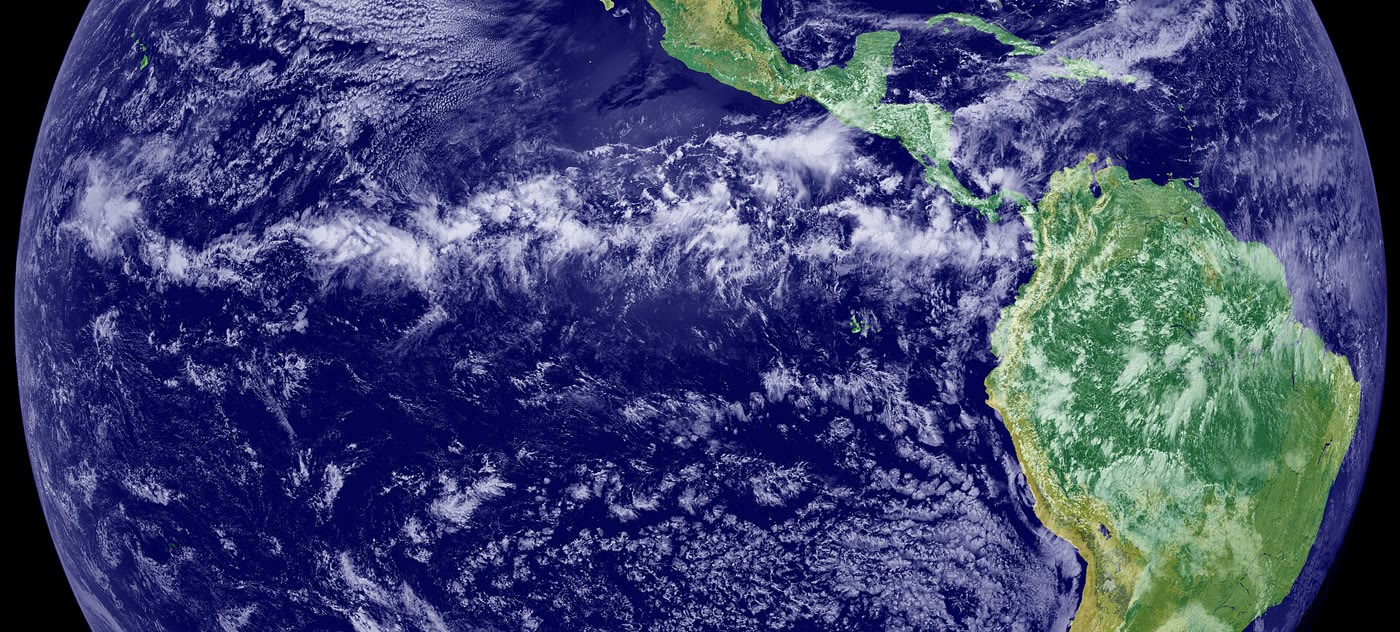
\includegraphics[width=0.8\linewidth]{images/book3/b1-itcz-goes.jpg}

{\small A \omterm{def:b1:atmospheric-circulation:itcz}{zona de convergência intertropical} sobre o Pacífico leste: uma linha de nuvens brilhantes
atravessando o oceano ao norte do equador, com a América Central e a do Sul à direita. A imagem
combina dados de nuvens do satélite geoestacionário GOES-11 com cores da cobertura do solo. (NASA
Earth Observatory, domínio público, via Wikimedia Commons.)}
\label{fig:b1:atmospheric-circulation:itcz-photo}
\end{omfigure}
% ledger: commons:itcz-goes

O ar convergente precisa subir, e o ar úmido ascendente forma nuvens: a ZCIT é o cinturão mais
chuvoso do planeta, e sua posição é traçada pela \omterm{def:b1:spherical-astronomy:geographic}{latitude} onde a precipitação zonal média atinge o
máximo. A ZCIT segue o Sol, com atraso. Na reanálise o máximo se desloca de \ang{12.8} S em fevereiro
para \ang{10.9} N em setembro; média sobre os doze meses ela fica a \ang{2.6} N. A média zonal esconde
grandes diferenças entre \omterm{def:b1:spherical-astronomy:geographic}{longitudes}: sobre o Pacífico leste da fotografia a faixa fica ao norte do
equador, e uma média zonal mistura essas faixas com outras que oscilam mais longe com as estações.
% ledger: data:b3-ncep (computed in figdata/bachelor-1/general_circulation.py)

\begin{omfigure}
\begin{tikzpicture}
\begin{axis}[omrecord, width=0.7\linewidth, height=5.2cm, xmin=0.5, xmax=12.5, ymin=-16, ymax=16,
  xlabel={mês}, ylabel={latitude (\unit{\degree})}, xtick={1,...,12},
  xticklabels={J,F,M,A,M,J,J,A,S,O,N,D}, ytick={-15,-10,...,15}]
% figdata/bachelor-1/general_circulation.py; ledger: data:b3-ncep
\addplot[black!40, domain=0.5:12.5] {0};
\addplot[omThm, line width=1.1pt, mark=*, mark size=1.6pt] table[x=month, y=lat] {figdata/out/bachelor-1-general_circulation-itcz.dat};
\end{axis}
\end{tikzpicture}

{\small A \omterm{def:b1:spherical-astronomy:geographic}{latitude} do máximo de precipitação zonal média, mês a mês, entre \ang{20} S e \ang{20} N: a
\omterm{def:b1:atmospheric-circulation:itcz}{zona de convergência intertropical} migra para o norte no verão do norte e para o sul no verão do sul,
dois ou três meses atrás do Sol. Reanálise~1 NCEP-NCAR, médias 1991--2020, dados fornecidos pelo NOAA
PSL.}
\label{fig:b1:atmospheric-circulation:itcz}
\end{omfigure}
% ledger: data:b3-ncep

Ao longo do próprio equador, onde $f = 0$, o ar se move diretamente pelo gradiente de pressão, e uma
circulação leste--oeste aparece sobre o Pacífico.

\begin{definition}[Circulação de Walker]\label{def:b1:atmospheric-circulation:walker}
A \emph{circulação de Walker}\index{circulação de Walker} é a célula de circulação leste--oeste da
atmosfera ao longo do Pacífico equatorial: o ar sobe sobre as águas quentes do oeste, em torno do
Continente Marítimo, escoa para leste em altitude, desce sobre o Pacífico leste e retorna para oeste
perto da superfície, com os \omterm{def:b1:atmospheric-circulation:winds}{alísios}.
\end{definition}
% ledger: climategov:walker

\begin{omfigure}
\begin{tikzpicture}[>={Stealth[length=2mm]}, font=\scriptsize]
  \fill[blue!12] (0,0) rectangle (11,0.45);
  \shade[left color=orange!45, right color=blue!12] (0,0) rectangle (6,0.45);
  \fill[brown!45] (-0.9,0) rectangle (0,0.6);
  \fill[brown!45] (11,0) rectangle (11.9,0.6);
  \node[anchor=north] at (-0.45,-0.05) {Marítimo};
  \node[anchor=north] at (-0.45,-0.35) {Continente};
  \node[anchor=north] at (11.45,-0.05) {Sul};
  \node[anchor=north] at (11.45,-0.35) {América};
  \node[anchor=north] at (5.5,-0.05) {oceano Pacífico equatorial};
  \node at (1.6,0.22) {água quente};
  \foreach \x in {0.6,1.2,1.8} \fill[black!20] (\x,2.6) circle (0.45);
  \foreach \x in {0.9,1.5} \fill[black!25] (\x,3.0) circle (0.4);
  \draw[line width=1.2pt, omThm, ->] (9.5,0.8) -- (2.0,0.8);
  \draw[line width=1.2pt, omThm, ->] (1.2,1.0) -- (1.2,3.0);
  \draw[line width=1.2pt, omThm, ->] (2.0,3.3) -- (9.5,3.3);
  \draw[line width=1.2pt, omThm, ->] (10.3,3.0) -- (10.3,1.0);
  \node[anchor=south] at (5.75,0.85) {alísios, de leste para oeste};
  \node[anchor=south] at (5.75,3.35) {escoamento de retorno em altitude, de oeste para leste};
  \node[anchor=west, align=left] at (1.6,1.8) {ar ascendente,\\chuva forte};
  \node[anchor=east, align=right] at (10.0,1.8) {ar descendente,\\seco};
\end{tikzpicture}

{\small A \omterm{def:b1:atmospheric-circulation:walker}{circulação de Walker} ao longo do Pacífico equatorial (esquemático; altura fora de escala):
ascendendo sobre o oeste quente, para leste em altitude, descendo no leste e voltando para oeste com
os \omterm{def:b1:atmospheric-circulation:winds}{alísios} perto da superfície.}
\label{fig:b1:atmospheric-circulation:walker}
\end{omfigure}
% ledger: climategov:walker

A \omterm{def:b1:atmospheric-circulation:walker}{circulação de Walker} não é estacionária. Quando ela se enfraquece, o movimento ascendente sobre o
Continente Marítimo se enfraquece e o ar ali pode até descer; quando se fortalece, a subida e a chuva
sobre o oeste aumentam. Essas oscilações, El~Niño e La~Niña, e as inversões sazonais das monções são
assunto do Livro~4. Ao longo das décadas desde 1980, a avaliação de 2021 do IPCC encontra um
fortalecimento \emph{muito provável} da \omterm{def:b1:atmospheric-circulation:walker}{circulação de Walker}, parecido com o estado de La~Niña, e um
deslocamento para oeste, com \emph{confiança média} quanto ao tamanho das mudanças.
% ledger: climategov:walker, ipcc:hadley-widening

\section{Correntes de jato}\label{sec:b1:atmospheric-circulation:jets}

\begin{definition}[Corrente de jato; jatos subtropical e da frente polar]\label{def:b1:atmospheric-circulation:jet}
Uma \emph{corrente de jato}\index{corrente de jato} é uma faixa estreita de vento forte, normalmente um
vento horizontal alto na troposfera, cuja posição muda de dia para dia. O \emph{jato subtropical}\index{jato subtropical}
sopra de oeste perto da borda polar da \omterm{def:b1:atmospheric-circulation:cells}{célula de Hadley}, em geral entre \ang{20} e \ang{30} de \omterm{def:b1:spherical-astronomy:geographic}{latitude}
a alturas de \qtyrange{12}{14}{km}. O \emph{jato da frente polar}\index{jato da frente polar} sopra
de oeste acima da fronteira entre ar polar e subtropical, entre cerca de \ang{50} e \ang{60}; é o núcleo
rápido dos \omterm{def:b1:atmospheric-circulation:winds}{ventos de oeste}, guiado pelas e guiando as depressões e \omterm{def:b1:atmospheric-circulation:cyclone}{anticiclones} das \omterm{def:b1:spherical-astronomy:geographic}{latitudes} médias.
\end{definition}
% ledger: nws:jets, noaajs:jet

\omterm{def:b1:atmospheric-circulation:jet}{Correntes de jato} costumam ser encontradas perto de \qty{9}{km}, podem passar de \qty{440}{km/h}, e
são mais fortes no inverno de cada hemisfério, quando o contraste de temperatura entre os trópicos e o
polo é maior. O \omterm{def:b1:atmospheric-circulation:jet}{jato subtropical} é o vento de momento angular de
\cref{prop:b1:atmospheric-circulation:angular-momentum}, domado pelos redemoinhos; ele fica na borda da
\omterm{def:b1:atmospheric-circulation:cells}{célula de Hadley}, perto de \ang{30} na média de inverno. O \omterm{def:b1:atmospheric-circulation:jet}{jato da frente polar} oscila para o norte e
para o sul com as depressões que passam, e a média sobre o globo o espalha: na média zonal do verão do
norte resta apenas um máximo fraco de \qty{21.6}{m/s} perto de \ang{42.5} N, e no verão do sul
\qty{29.9}{m/s} perto de \ang{47.5} S. Por que o vento aumenta com a altura onde a temperatura cai em
direção ao polo, o vento térmico, é mostrado no Livro~5.
% ledger: noaajs:jet, nws:jets, data:b3-ncep-circ (computed in figdata/bachelor-1/general_circulation.py)

\section{Exercícios}

\begin{exercise}[$\star$]\label{exo:b1:atmospheric-circulation:1}
Tome $\Omega = \qty{7.292e-5}{rad.s^{-1}}$. (a)~Calcule o \omterm{def:b1:atmospheric-circulation:coriolis-parameter}{parâmetro de Coriolis} a \ang{0}, \ang{30},
\ang{45} e \ang{90} N. (b)~Calcule a aceleração horizontal de Coriolis de um vento de \qty{10}{m/s} a
\ang{45} N e compare-a com $g =
\qty{9.81}{m.s^{-2}}$. (c)~Em que direção ela aponta se o vento sopra para o norte?
% ledger: earth:Trot
\end{exercise}

\begin{exercise}[$\star$]\label{exo:b1:atmospheric-circulation:2}
Duas isóbaras de \qty{4}{hPa} de distância estão a \qty{400}{km} de distância ao nível do mar, onde
$\rho =
\qty{1.225}{kg.m^{-3}}$. (a)~Calcule a aceleração devida à \omterm{def:b1:atmospheric-circulation:pgf}{força do gradiente de pressão}. (b)~Se nada
mais atuasse, quanto tempo levaria para acelerar um ar parado a \qty{10}{m/s}? (c)~Compare essa
aceleração com a aceleração de Coriolis de um vento de \qty{10}{m/s} a \ang{45} N, e diga o que isso sugere.
% ledger: ussa76:sea-level, earth:Trot
\end{exercise}

\begin{exercise}[$\star$]\label{exo:b1:atmospheric-circulation:3}
A \ang{40} N, isóbaras de \qty{4}{hPa} de distância estão a \qty{250}{km} de distância; tome $\rho =
\qty{1.225}{kg.m^{-3}}$. (a)~Calcule o \omterm{def:b1:atmospheric-circulation:geostrophic}{vento geostrófico} em \unit{m/s} e em nós (\qty{1}{kn} =
\qty{0.5144}{m/s}). (b)~A baixa fica ao sul. De que direção sopra o vento? (c)~Descreva a barbela do
vento (haste e penas) que um meteorologista desenharia.
% ledger: ussa76:sea-level, earth:Trot
\end{exercise}

\begin{exercise}[$\star$]\label{exo:b1:atmospheric-circulation:4}
As médias anuais da reanálise dão, perto do solo, o vento para leste \qty{-3.5}{m/s} a \ang{15} N,
\qty{-4.4}{m/s} a \ang{15} S, \qty{+1.9}{m/s} a \ang{45} N e \qty{+6.5}{m/s} a \ang{45} S, e a pressão
ao nível do mar \qty{1011.8}{hPa} a \ang{15} N, \qty{1016.8}{hPa} a \ang{30} N e \qty{1015.8}{hPa} a
\ang{45} N. (a)~Dê o nome do cinturão de vento em cada uma das quatro \omterm{def:b1:spherical-astronomy:geographic}{latitudes}. (b)~Explique o sinal de
cada vento com o ramo de superfície de uma célula. (c)~Onde fica a \omterm{def:b1:atmospheric-circulation:cells}{alta subtropical} do Hemisfério Norte
segundo essas pressões?
% ledger: data:b3-ncep-circ
\end{exercise}

\begin{exercise}[$\star\star$]\label{exo:b1:atmospheric-circulation:5}
Um gradiente de pressão de \qty{2}{hPa} por \qty{500}{km}, com $\rho =
\qty{1.225}{kg.m^{-3}}$, é encontrado a \ang{60}, \ang{50}, \ang{30}, \ang{20}, \ang{10} e \ang{5} N.
(a)~Calcule o \omterm{def:b1:atmospheric-circulation:geostrophic}{vento geostrófico} em cada \omterm{def:b1:spherical-astronomy:geographic}{latitude}. (b)~Os ventos reais dos trópicos profundos raramente
passam de alguns metros por segundo sobre gradientes desse tipo. Explique por que o \omterm{def:b1:atmospheric-circulation:geostrophic}{equilíbrio
geostrófico} falha perto do equador, usando o tempo $1/f$ que a força de Coriolis leva para girar o vento.
% ledger: ussa76:sea-level, earth:Trot
\end{exercise}

\begin{exercise}[$\star\star$]\label{exo:b1:atmospheric-circulation:6}
(a)~Com \cref{prop:b1:atmospheric-circulation:angular-momentum}, calcule o vento de um anel de ar que
deixa o equador em repouso, a \ang{10}, \ang{15}, \ang{20} e \ang{30}; tome $\Omega a_\oplus = \qty{464.6}{m/s}$. (b)~O mesmo para um anel que começa em repouso a \ang{10}, \ang{15}, \ang{20} e
\ang{30}. (c)~O ramo ascendente da \omterm{def:b1:atmospheric-circulation:cells}{célula de Hadley} se espalha por \omterm{def:b1:spherical-astronomy:geographic}{latitudes} em vez de ficar exatamente
no equador. Como isso muda o jato previsto?
% ledger: earth:Trot, earth:Rmean
\end{exercise}

\begin{exercise}[$\star\star$]\label{exo:b1:atmospheric-circulation:7}
(a)~Um navio no Hemisfério Norte tem o vento de sudoeste. Usando a lei de Buys Ballot, onde está o
centro de baixa pressão? (b)~Um navio no Hemisfério Sul tem o vento de noroeste. Onde está a baixa?
(c)~Perto do solo o vento cruza as isóbaras em direção à baixa pressão. Isso muda sua resposta a (a),
girando a direção da baixa no sentido horário ou anti-horário?
% ledger: skybrary:buys-ballot
\end{exercise}

\begin{exercise}[$\star\star$]\label{exo:b1:atmospheric-circulation:8}
(a)~Calcule a massa de ar entre o equador e \ang{30} N e entre os níveis de pressão \qty{1000}{hPa} e
\qty{100}{hPa}, com $a_\oplus = \qty{6371}{km}$ e $g = \qty{9.81}{m.s^{-2}}$. (b)~Na média anual a \omterm{def:b1:atmospheric-circulation:cells}{célula
de Hadley} norte da reanálise transporta \qty{8.7e10}{kg/s}. Quanto tempo levaria para fazer essa massa
passar pela célula uma vez? (c)~A mesma pergunta para a célula do inverno do norte, \qty{21.4e10}{kg/s}.
% ledger: earth:Rmean, data:b3-ncep-circ
\end{exercise}

\begin{exercise}[$\star\star$]\label{exo:b1:atmospheric-circulation:9}
Suponha que sob uma \omterm{def:b1:atmospheric-circulation:cells}{alta subtropical} o ar desce a \qty{1}{cm/s}, e que ele é insaturado. (a)~Quanto ele
desce em um dia? (b)~Quanto ele aquece em um dia, se nada mais atuar, com o \omterm{def:b1:fluid-envelopes-structure:lapse-rate}{gradiente adiabático seco}
de \qty{9.8}{K/km}? (c)~O ar não aquece tanto assim dia após dia. Qual processo de
\cref{ch:b1:radiation-heat-transport} equilibra o aquecimento? (d)~Por que muitos dos grandes desertos
quentes se encontram sob essas altas?
% ledger: nws:dalr
\end{exercise}

\begin{exercise}[$\star\star\star$]\label{exo:b1:atmospheric-circulation:10}
A \ang{50} N, tome $f = \qty{1.117e-4}{s^{-1}}$ e isóbaras circulares de raio $r = \qty{500}{km}$
(\cref{rem:b1:atmospheric-circulation:gradient}). (a)~Em torno de uma baixa onde o \omterm{def:b1:atmospheric-circulation:geostrophic}{vento geostrófico}
seria \qty{15}{m/s}, resolva $V^2/r + fV =
f|\vec v_g|$ para o vento de gradiente $V$. (b)~Em torno de uma alta, mostre que $V^2/r - fV + f
|\vec v_g| = 0$ tem solução apenas se $|\vec v_g| \leq fr/4$, e calcule esse limite. (c)~O que (b)
implica para o espaçamento das isóbaras perto do centro de um \omterm{def:b1:atmospheric-circulation:cyclone}{anticiclone}, comparado com uma depressão?
\end{exercise}

\begin{exercise}[$\star\star\star$]\label{exo:b1:atmospheric-circulation:11}
(a)~Mostre que, para $\varphi$ pequeno (em radianos), o vento de um anel que deixa o equador em repouso
é $u \approx \Omega a_\oplus\varphi^2$. (b)~Compare a aproximação com a fórmula exata a \ang{10}, com
$\Omega a_\oplus = \qty{464.6}{m/s}$. (c)~O vento zonal médio anual da reanálise a \qty{200}{hPa} atinge o
máximo de \qty{27.0}{m/s} perto de \ang{35} N. A que \omterm{def:b1:spherical-astronomy:geographic}{latitude} o anel atingiria essa velocidade? (d)~O que
a resposta diz sobre até onde o argumento do momento angular pode ser confiável?
% ledger: earth:Trot, earth:Rmean, data:b3-ncep-circ
\end{exercise}

\begin{exercise}[$\star\star\star$]\label{exo:b1:atmospheric-circulation:12}
A precipitação zonal média da reanálise atinge o máximo nas seguintes \omterm{def:b1:spherical-astronomy:geographic}{latitudes}, de janeiro a
dezembro: \ang{-10.5}, \ang{-12.8}, \ang{-5.8}, \ang{-4.6}, \ang{5.5}, \ang{7.3}, \ang{8.6}, \ang{10.4},
\ang{10.9}, \ang{9.1}, \ang{7.4}, \ang{6.2} (negativo: sul). (a)~Calcule a média anual e a amplitude.
(b)~A \omterm{def:b1:spherical-astronomy:geographic}{latitude} subsolar é extrema em junho e dezembro. Com quantos meses a ZCIT se atrasa em relação a
ela, e o que no sistema climático pode armazenar calor para causar esse atraso? (c)~Suponha que sobre um
oceano a ZCIT fique ao norte do equador o ano inteiro. Explique como a média zonal ainda pode cruzar o
equador.
% ledger: data:b3-ncep
\end{exercise}

\section{Problema: lendo um mapa do tempo de latitude média}

\begin{problem}[{Problema de fim de semana --- o vento em uma estação perto de \ang{50} N}]
\label{pb:b1:atmospheric-circulation:1}
% values: calc/ch28.py (invented map; jet from data:b3-ncep-circ)
Um mapa do tempo do Atlântico Norte mostra, perto de uma estação P a \ang{50} N, isóbaras retas de
oeste para leste, a cada \qty{4}{hPa}, com as pressões mais baixas ao norte. P fica entre as isóbaras
de \qty{1004}{hPa} e \qty{1008}{hPa}, que estão a \qty{250}{km} de distância ali; sua pressão ao nível
do mar é \qty{1006}{hPa} e sua temperatura do ar \qty{10}{\degreeCelsius}. O mapa é inventado, mas seus
números são típicos. Use $\Omega = 2\pi/(\qty{23.9345}{h})$, $a_\oplus = \qty{6371}{km}$, $R_d =
\qty{287.05}{J.kg^{-1}.K^{-1}}$ para o ar seco, \qty{1}{kn} = \qty{0.514444}{m/s}.

\medskip
\noindent\textbf{Parte I --- O gradiente de pressão e o vento geostrófico.}
\begin{enumerate}
  \item Calcule a densidade do ar em P com a lei dos gases ideais.
  \item Calcule o gradiente de pressão horizontal em P, em \unit{Pa.m^{-1}}.
  \item Calcule a aceleração devida à \omterm{def:b1:atmospheric-circulation:pgf}{força do gradiente de pressão}.
  \item Calcule $\Omega$ e o \omterm{def:b1:atmospheric-circulation:coriolis-parameter}{parâmetro de Coriolis} a \ang{50} N.
  \item Calcule a velocidade do \omterm{def:b1:atmospheric-circulation:geostrophic}{vento geostrófico} em P.
  \item Exprima-a em nós e em \unit{km/h}.
  \item Mostre que o tempo que a \omterm{def:b1:atmospheric-circulation:pgf}{força do gradiente de pressão} sozinha levaria para trazer ar parado
        à velocidade geostrófica é $1/f$, e calcule-o, junto com o tempo $2\pi/f$ que a força de Coriolis
        leva para girar um vento por um círculo completo.
\end{enumerate}

\medskip
\noindent\textbf{Parte II --- Direção e hemisfério.}
\begin{enumerate}[resume]
  \item Em que direção a \omterm{def:b1:atmospheric-circulation:pgf}{força do gradiente de pressão} aponta em P? Em que direção sopra o \omterm{def:b1:atmospheric-circulation:geostrophic}{vento
        geostrófico}, e de que \omterm{def:b1:spherical-astronomy:horizontal}{azimute} ele vem?
  \item Verifique sua resposta com a lei de Buys Ballot.
  \item Descreva a barbela do vento desenhada em P: a direção da haste, o número de penas e o lado em
        que elas ficam.
  \item Suponha as mesmas isóbaras, com a baixa ao norte, encontradas a \ang{50} S. De que direção
        sopraria o vento?
  \item Com a mesma densidade e o mesmo gradiente de pressão, calcule o \omterm{def:b1:atmospheric-circulation:geostrophic}{vento geostrófico} a \ang{30} N
        e \ang{60} N.
  \item Calcule-o a \ang{5} N. O resultado é crível? Explique.
\end{enumerate}

\medskip
\noindent\textbf{Parte III --- O vento no solo.} Um anemômetro em P mede um vento de \qty{9.0}{m/s}
cruzando as isóbaras a \ang{25} em direção à baixa pressão.
\begin{enumerate}[resume]
  \item Calcule a razão entre o vento observado e o \omterm{def:b1:atmospheric-circulation:geostrophic}{vento geostrófico}, e as componentes do vento
        observado ao longo e através das isóbaras.
  \item De que \omterm{def:b1:spherical-astronomy:horizontal}{azimute} sopra o vento observado?
  \item No modelo de arrasto linear de \cref{prop:b1:atmospheric-circulation:friction}, qual constante
        de tempo $\tau$ dá o ângulo observado, e que velocidade o modelo prevê então? Compare com a
        observação.
  \item Em torno de uma depressão de raio \qty{500}{km}, suponha que o ar da camada mais baixa, de um
        quilômetro, flui para dentro em toda parte com a componente através das isóbaras da questão~14 e
        a densidade da questão~1. Calcule a massa de ar que entra na depressão por segundo.
  \item Esse ar deve sair pelo topo da camada. Calcule a velocidade média ascendente ali, em
        \unit{m/s} e em metros por dia.
  \item À taxa adiabática seca de \qty{9.8}{K/km}, quanto esfria o ar ascendente em um dia? Que tempo
        se segue, e o que aconteceria sob um \omterm{def:b1:atmospheric-circulation:cyclone}{anticiclone}?
\end{enumerate}

\medskip
\noindent\textbf{Parte IV --- O jato acima.} O vento zonal médio a \qty{200}{hPa} no inverno do norte
atinge o máximo de \qty{42.3}{m/s} perto de \ang{30} N (médias da reanálise 1991--2020).
\begin{enumerate}[resume]
  \item Calcule a velocidade para leste do solo no equador e a \ang{30} N.
  \item Um anel de ar deixa o equador em repouso em altitude e conserva seu momento angular. Calcule seu
        vento a \ang{20} N e a \ang{30} N.
  \item A mesma pergunta a \ang{30} N para um anel que começa em repouso a \ang{10} N.
  \item De que fator o anel da questão~21 ultrapassa o jato observado a \ang{30} N? Dê duas razões pelas
        quais o jato real é mais lento.
  \item Calcule a razão entre o momento angular absoluto por unidade de massa do jato observado a
        \ang{30} N e o do ar em repouso no equador. Que fração foi perdida no caminho?
  \item Qual é a velocidade do \omterm{def:b1:atmospheric-circulation:geostrophic}{vento geostrófico} em P, em metros por segundo, e como o vento medido no
        solo se compara com ela?
\end{enumerate}
\end{problem}
